\documentclass[titlepage]{article}
\usepackage{babel}
\usepackage{amsmath}
\usepackage{amssymb}
\usepackage{amsthm}
\usepackage{multicol} %spalten in seite
\usepackage{graphicx} %bilder einfügen
\usepackage[normalem]{ulem} %durchstreichen
\usepackage{tabto} %tabulator mit \tab
\usepackage{hyperref}
\usepackage{tikz}
\usetikzlibrary{automata, arrows.meta, positioning} % automaten zeichnen
\usetikzlibrary{shapes.geometric}
\usepackage{wasysym}
\usepackage{bbm}
\usepackage{bbold}
\usepackage{xcolor}
\usepackage[T1]{fontenc}
\usepackage{mathrsfs}  
\usepackage[utf8]{inputenc}
\usepackage{listings} %quellcode
\pagestyle{plain}
\pagenumbering{arabic}
\renewcommand{\arraystretch}{1.3} %vertikaler abstand von tabellen
\newcommand{\n}{\newline}
\usepackage[left=20mm, right=15mm, top=25mm, bottom=7mm, paper=a4paper]{geometry}


\renewcommand{\contentsname}{Inhaltsverzeichnis}

\renewcommand{\]}{\right]}
\renewcommand{\[}{\left[}
\renewcommand{\)}{\right)}
\renewcommand{\(}{\left(}
\renewcommand{\|}{\;|\;}
\usetikzlibrary {arrows.meta,automata,positioning,shadows}


\begin{document}
	
	\begin{center}
		
\begin{tikzpicture}
			\draw (0,0) node[draw, rectangle]{\textsc{Wintersemester 2022/23}};
		\end{tikzpicture}
		\hrulefill\\
		\begin{center}
			\LARGE\textsc{Automaten und Berechenbarkeit - Übung 02} \normalsize\\
		\end{center}
		\hrulefill
		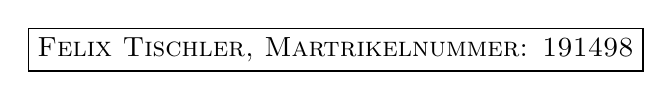
\begin{tikzpicture}
			\draw (0,0) node[draw, rectangle]{\textsc{Felix Tischler, Martrikelnummer: 191498}};
		\end{tikzpicture}
		\date{\today}
	\end{center}
	
	
	
	
	
	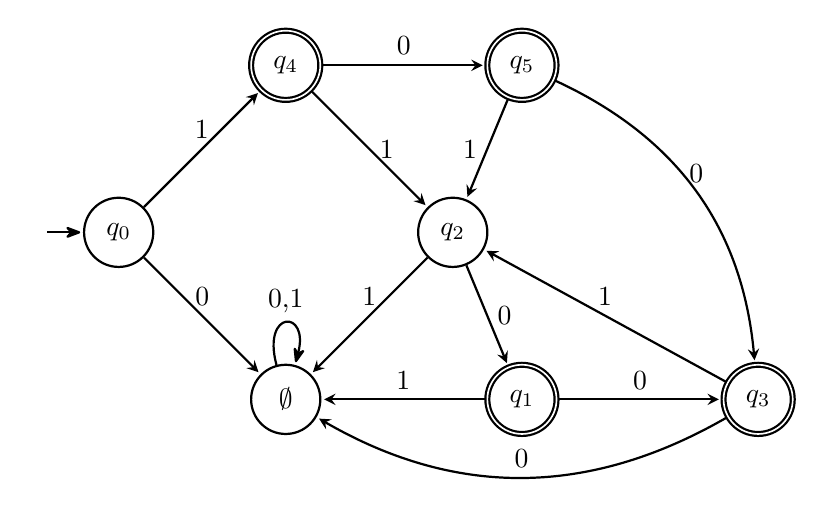
\begin{tikzpicture}[shorten >=1pt,node distance=3cm,on grid,>={Stealth[round]},thick]
		
		\node (q0) [state, initial, initial text = {}] {$q_0$};
		\node (q4) [state, accepting, above right of = q0] {$q_4$};
		\node (empty) [state, below right of = q0] {$\emptyset$};
		\node (q1) [state, accepting, right of = empty] {$q_1$};
		\node (q2) [state, below right of = q4] {$q_2$};
		\node (q3) [state, accepting, right of = q1] {$q_3$};
		
		\node (q5) [state, accepting, right of = q4] {$q_5$};
		
		\path [-stealth, thick]
		(empty) edge [loop above] node {0,1} (empty)
		(q0) edge node [above] {0} (empty)
		(q0) edge node [above] {1} (q4)
		
		(q1) edge node [above] {0} (q3)
		(q1) edge node [above] {1} (empty)
		
		(q2) edge node [right] {0} (q1)
		(q2) edge node[above] {1} (empty)
		
		(q3) edge [bend left] node [above] {0} (empty)
		(q3) edge node [above] {1} (q2)
		
		(q4) edge node [above] {0} (q5)
		(q4) edge node [right] {1} (q2)
		
		(q5) edge [bend left] node [above] {0} (q3)
		(q5) edge node [left] {1} (q2);
	\end{tikzpicture}

\end{document}